\section{Bin Packing}
\label{binpacking}

In the classic version of the problem, we are given items of different sizes and need to pack them into as few bins as possible. In the online stochastic version, items arrive one at a time and item sizes are drawn from an unknown distribution. 
Many resource allocation problems in Operations Research and Computer Science face uncertain future demand, and can be cast as variants of the online bin packing problem. In warehouse and transportation operations, variants of bin packing can be seen in: the order assignment problem (where we assign orders to fulfillment resources), the tote packing problem (where we fill items as they arrive into totes for shipment), and the trailer truck packing problem. In computing, bin packing problems arise in datacenters where virtual machines must be placed on servers, thus allocating memory and computing to processes within a machine.


%For instance, in the cutting stock problem, a manufacturer produces cables of fixed lengths, customer orders that with specific cable lengths arrive and must be served online from the available inventory.  The goal is to serve the demand while minimizing the rate of production of cables. In appointment scheduling, requests for appointments arrive online and must be scheduled in a future day with available slots. Here appointments correspond to items, and the office hours during a working day correspond to bins. 

%In this problem, customers orders arrive online and must be assigned to a ship method that connects an Amazon FC to the customer's location. For candidate each assignment, the order items would utilize our transportation resources (truck/plane space, labor). The task is to fulfill all orders while utilizing the least number of transportation resources.
 
\ifx 3d bin packing has many applications within Amazon operations from packing of picked items into totes to the packing of packages onto trailers. The need to use as few bins as possible directly translates into cost savings. \emph{Bharath} can you write about the VM
\fi

\subsection{Problem Formulation} \label{sec: bin_packing_prob_form}
In the stochastic bin packing problem, items arrive online, one in each time period $t$, with $t \in \{1, \ldots, T\}$. Items can be of different types $j \in \{1,...,J\}$. The size of type $j$ is $s_j$ and the probability that an item is of type $j$ is $p_j$. Without loss of generality, we assume item types are indexed in the increasing order of their size: $s_1 < s_2 < ... < s_J$. Upon arrival, the item needs to be packed into one of the bins, each with size $B$ (we assume that $s_J < B < \infty$). A packing is considered feasible if the total size of the items packed in each bin does not exceed the bin size. The task is to find a feasible packing that minimizes the number of bins used to pack all of the items that arrive within the time horizon. We assume the item sizes $s_j$ and bin size $B$ are integers. We assume the number of bins one can open is unlimited and denote the sum of item sizes in a bin $k$ as \emph{level} $h_{k}$. After $t$ items have been packed, we denote the number of bins at some level $h$ as $N_h(t)$, where $h \in \{1,...,B\}$. The formulation of online bin packing is from \cite{gupta2012online}. 

It can be shown that minimizing the number of non-empty bins is equivalent to minimizing the total waste (i.e. empty space) in the partially filled bins.  In real applications (e.g. packing trucks, or virtual machines), there is a dollar-value cost associated with the consumption of these resources, so at any time horizon our objective is to minimize total waste $\sum_{t=0}^{T} W(t)$, where

\begin{equation}
\label{waste}
W(t) \triangleq \sum_{h=1}^{B-1} N_h(t)(B-h) 
\end{equation}

\noindent We use $W^{A}_{F}(t)$ to denote the total waste after step $t$ of algorithm $A$ when the input samples come from distribution $F$. For RL, we define the cumulative reward up to time step $t$ to be $W^{RL}_{F}(t)$. \cite{courcobetis1990stability} showed that any discrete distribution falls into one of three categories based on expected distribution $E[W^{OPT}_{F}(t)]$.
\begin{enumerate}[topsep=0pt,itemsep=-1ex,partopsep=1ex,parsep=1ex]
	\item Linear waste (LW): $E[W^{OPT}_{F}(t)] = \Theta(t)$, e.g. $B = 9$, two item types of size $\{2,3\}$ with probability $\{0.8, 0.2\}$ respectively.
	\item Perfectly Packable (PP):  $E[W^{OPT}_{F}(t)] = \Theta(\sqrt{t})$, e.g.  $B = 9$, two item types of size $\{2,3\}$ with probability $\{0.75, 0.25\}$ respectively.
	\item PP with bounded waste (BW): $E[W^{OPT}_{F}(t)] = \Theta(1)$, e.g. $B = 9$, two item types of size $\{2,3\}$ with probability $\{0.5, 0.5\}$ respectively.
\end{enumerate}
We will train an RL policy for each of the three distribution types and compare our policy to the appropriate baseline.


\subsection{Related Work}
Bin packing is a well-studied problem in the operations research and computer science literature. 
%Some applications include: loading trucks subject to weight/volume restrictions, to packing television commercials into station breaks, to stock-cutting problems, where items of varying lengths must be cut from some raw materials, e.g. cable, lumber, or paper of a standard size. 
The problem is already NP-hard in its basic form. As a result, many of the classical approaches to bin packing analyze the performance of approximation algorithms. We refer the readers to the survey \cite{Coffmanetal2013} for algorithmic approaches to classical bin packing and its generalizations.   

For online bin packing, a simple heuristic -- Best Fit -- is known to use at most $1.7$ times the optimal number of bins in the worst case \cite{Johnsonetal1974}. Best Fit places an item in a bin where, if the item were to be packed, would leave the least amount of space.
%This paper focuses on the asymptotic performance of online stochastic bin packing. Many research papers in this vein analyze the performance of common (distributional agnostic) heuristics such as First Fit and Best Fit, and on specific distributions such as uniform \cite{Shor:1986}\cite{Leighton:1986}\cite{coffmanetal1991}\cite{Kenyon1998}\cite{Albers1998} and skewed uniform \cite{KenyonMitzen2000}. A few papers also identify an optimal policy for specific item size distributions, e.g. \cite{Shor1991}. 
%For asymptotic analysis, the Sum of Squares (SS) heuristic \cite{csirik2006sum} is arguably the state-of-the-art bin packing policy when item sizes $\{s_j\}$ and bin size $B$ are integer. It is distribution agnostic and nearly universally optimal (up to constant factors) for different types of distributions.
%In \cite{csirik2006sum}, it is shown that SS has $O(\sqrt{t})$ waste for PP distribution, matching the optimal. For BW distributions, the waste of SS is $O(\log t)$, which can be reduced to $O(1)$ by learning the support of the distribution. For LW, SS is suboptimal by an additive constant factor i.e. $\Theta(t)$. The sub-optimality can be reduced by learning the item size distribution and solving a LP to fine-tune the heuristic. \cite{gupta2012online} proposed heuristics to obtain $\Theta(\sqrt{t})$ additive sub-optimality for all distributions, inspired by approximate interior-point algorithms for convex optimization.
Another competitive heuristic is Sum of Squares (SS) heuristic \cite{csirik2006sum}. In particular, SS is proven to be asymtotically optimal (up to constants) as the episode length gets large.

The simple heuristics described above are distribution agnostic. More sophisticated algorithms learn an empirical estimate of the item size distribution, leverage such distribution to solve a linear program, and use its dual to guide the online policy \cite{AdelmanNem1999}\cite{RheeTalagrand1993}\cite{IyengarSigman2004}. This approach has been used to solve online packing and covering problems~\cite{GuptaMolinaro2014}\cite{AgrawalDevanur2015}.

%\textcolor{blue}{RL related work}

\subsection{Baseline Algorithms}
We use the Sum of Squares (SS) heuristic and Best Fit (BF) as our baseline algorithm. 
%For the integral item sizes and bin size problem, SS heuristic is nearly universally optimal for all item size distributions and almost distribution-agnostic. 
When the $t$th item of size $s$ arrives, SS picks a bin of level $h^*$ that minimizes the value of the following sum-of-squares potential:

\begin{equation}
\sum_{h=1}^{B-1} (N_{h}(t))^2 \label{SOS eq}
\end{equation}

\noindent It can be shown that minimizing (\ref{SOS eq}) is equivalent to minimizing:
\begin{equation}
h^* = \underset{h:N_h(t-1)>0 \ \text{and} \ h+s \leq B}{\arg\min} [N_{h+s}(t-1) - N_h(t-1)], \label{SOS eq1}
\end{equation}

\noindent where, $N_0 = N_B = 0$. Intuitively, SS tries to equalize the number of bins at each level. Due its simplicity, we implemented (\ref{SOS eq1}) version of SS.

BF selects a bin at the highest level that can still fit the item:
\begin{equation}
h^* = \underset{h:N_h(t-1)>0 \ \text{and} \ h+s \leq B}{\arg\max} h
\end{equation}
\subsection{Reinforcement Learning Formulation}
We formulate this as an MDP, where the state $S_t \in \mathcal{S}$ is current item size $s_j$ and the number of bins at each level: $N_h(t)$, where $h \in \{1,...,B\}$. The action $A$ is to pick a bin level which can fit the item.  Thus, the number of actions possible is $B$ with one action for each level and action 0 corresponds to opening a new bin. Initially, all the bins are empty. The reward $R_t$ is the negative of incremental waste as each item is put into a bin. If the item is put into an existing bin, the incremental waste will reduce by item size. If the item is put into a new bin, the waste increases by the empty space left in the new bin. We mask the invalid actions such as picking a level for which bins do not exist yet. We describe our environment in detail in Appendix \ref{sec:bin_packing_gym}.
%In that case, we shape the reward by assigning a high negative penalty (-100 in our experiments) and terminating the episode. Alternative reward shaping strategies are an important direction of future research.

\subsection{Reinforcement Learning Algorithm}
We use the Proximal Policy Optimization (PPO) algorithm~\cite{schulman2017proximal}. PPO is an actor-critic algorithm~\cite{konda2000actor}, where the actor is represented by a policy network and takes the environment state as input and produces an action as the output. The critic is represented by a value network and takes the environment state as input and predicts the cumulative discounted reward that will be obtained from this state. Intuitively, the actor tells the agent how to act and the critic informs the agent how good an action was. The two neural networks are initialized with random weights, i.e. the agent takes random actions, and the agent interacts with the environment to generate a dataset of tuples: $(S_t, A_t, R_t, S_{t+1})$. The dataset is used to update the weights of the two neural networks. The updated neural networks are used to interact with the environment to generate more data and the cycle continues until training stops. We refer the reader to the original paper~\cite{schulman2017proximal} for a formal explanation of the algorithm.

We use a two-layer neural network with 256 hidden nodes each. The input to both policy and value network is the state, the output of the policy network is a vector giving the probabilities of taking any action in the action space, and the output of the value network is predicted value. During training, the agent explores the state space by sampling from the probability distribution of the actions generated by the policy network. During evaluation, the agent takes the action with the highest action probability. We mask actions by reducing the probability of invalid actions to 0. Appendix \ref{appendix:bin_size_hp} lists the hyperparameters we use. 




\subsection{Results}
For each sample item size distribution (BW, PP, LW), we train the RL algorithm (PPO) and compare to the baseline algorithms (SS and BF).  We consider two variations, bin size of 9 with distributions listed in section \ref{sec: bin_packing_prob_form}, and bin size of 100 and the following item size distribution:

\begin{enumerate}[topsep=0pt,itemsep=-1ex,partopsep=1ex,parsep=1ex]
\item item sizes: $[1, 2, 3, 4, 5, 6, 7, 8, 9]$
\item item probabilities for BW: \\ $[0.14, 0.10, 0.06, 0.13, 0.11, 0.13, 0.03, 0.11, 0.19]$
\item item probabilities for PP: \\ $[0.06, 0.11, 0.11, 0.22, 0, 0.11, 0.06, 0, 0.33]$
\item item probabilities for LW: $[0, 0, 0, 1/3, 0, 0, 0, 0, 2/3]$.
\end{enumerate}
We use a single machine with 4 GPUs and 32 CPUs for our experiments. At a high level, by the end of training RL outperforms or matches the baseline irrespective of distribution, and converges to a sensible learned policy.

%\begin{figure}[h!]
%	\centering
%	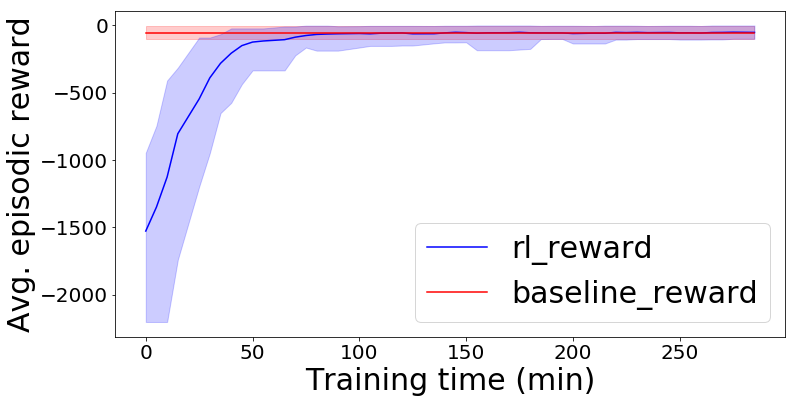
\includegraphics[width=1\linewidth]{images/bin_packing_rl_vs_baseline_bounded_waste_binsize_100.png}
%	\caption{RL vs baseline for BW distribution}
%	\label{fig:bin_packing_BW_dist1}
%\end{figure}
%
%\begin{figure}[h!]
%	\centering
%	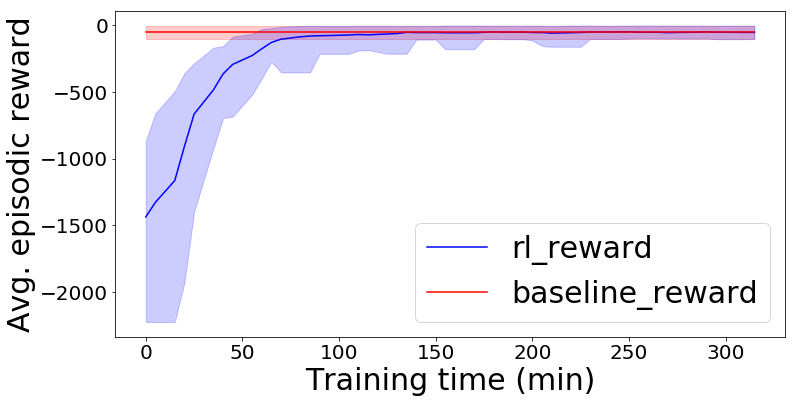
\includegraphics[width=1\linewidth]{images/bin_packing_rl_vs_baseline_perfect_pack_binsize_100.png}
%	\caption{RL vs baseline for PP distribution}
%	\label{fig:bin_packing_PP_dist1}
%\end{figure}
%
%\begin{figure}[h!]
%	\centering
%	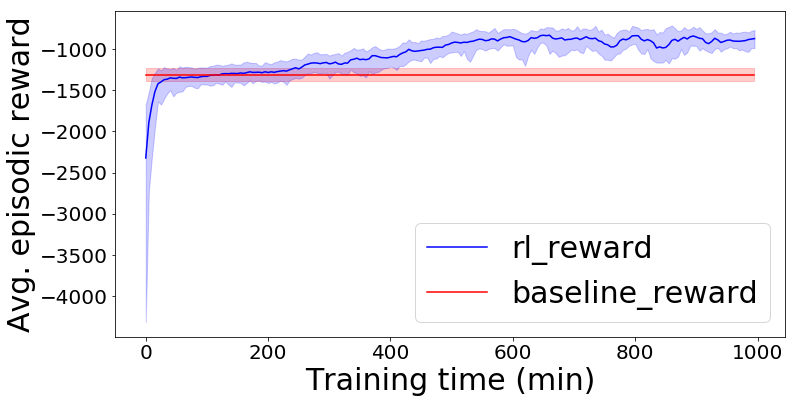
\includegraphics[width=1\linewidth]{images/bin_packing_rl_vs_baseline_linear_waste_binsize_100.png}
%	\caption{RL vs baseline for LW distribution}
%	\label{fig:bin_packing_LW_dist1}
%\end{figure}

\begin{figure*}
	\centering
	\begin{subfigure}[b]{0.33\textwidth}
		\centering
		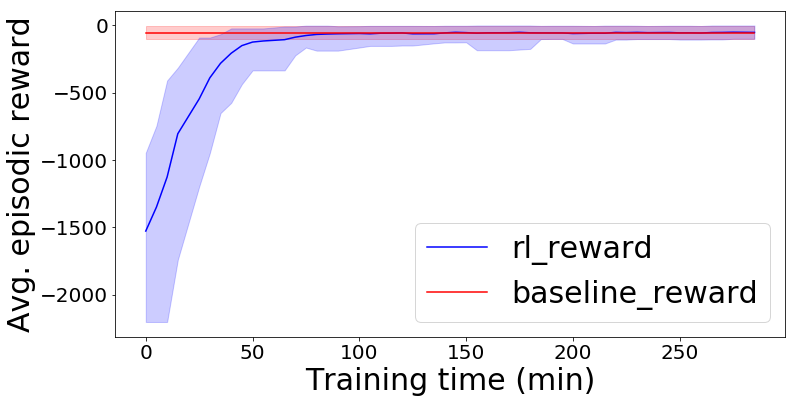
\includegraphics[width=\textwidth]{images/bin_packing_rl_vs_baseline_bounded_waste_binsize_100.png}
		\caption{RL vs baseline for BW distribution}
		\label{fig:bin_packing_BW_dist1}
	\end{subfigure}
	\hfill
	\begin{subfigure}[b]{0.33\textwidth}
		\centering
		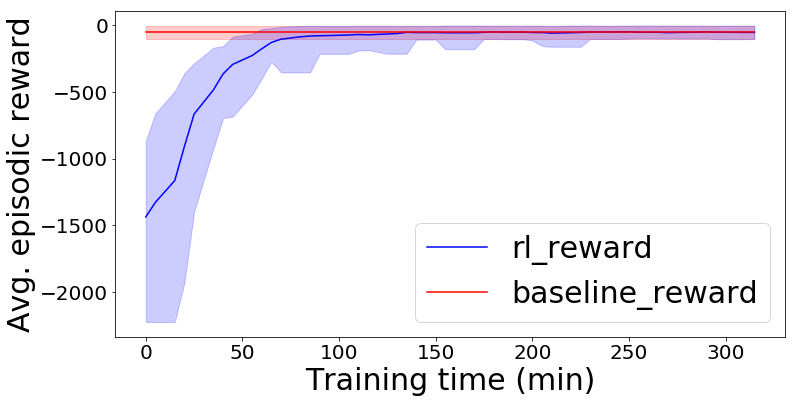
\includegraphics[width=\textwidth]{images/bin_packing_rl_vs_baseline_perfect_pack_binsize_100.png}
		\caption{RL vs baseline for PP distribution}
		\label{fig:bin_packing_PP_dist1}
	\end{subfigure}
	\hfill
	\begin{subfigure}[b]{0.33\textwidth}
		\centering
		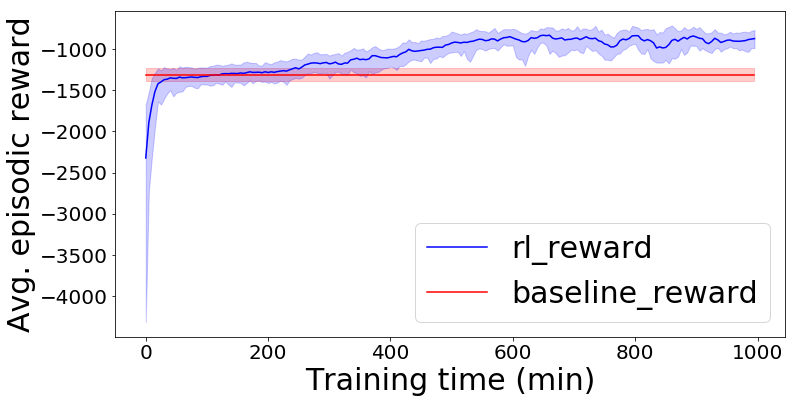
\includegraphics[width=\textwidth]{images/bin_packing_rl_vs_baseline_linear_waste_binsize_100.png}
		\caption{RL vs baseline for LW distribution}
		\label{fig:bin_packing_LW_dist1}
	\end{subfigure}
	\caption{Comparison of episodic rewards between RL and Best Fit baseline during training.}
	\label{fig:RLvsBF_binpacking}
		\vspace{-1em}
\end{figure*}


Figure \ref{fig:RLvsBF_binpacking} plots the reward function of the RL policy in training (blue) vs the Best Fit baseline (red) for bin size 100 and different item size distributions (BW, PP, and LW) as a function of training time (measured in minutes). The solid lines represent the mean reward of each policy, and the shaded bands represent the min/max rewards. By the end of training, RL either matches or outperforms the baseline policy for all three item size distributions. In particular, the reward gap between RL and baseline is the largest for LW distribution (which is expected, as both BF and SS are known to be suboptimal for LW distribution). %The min reward of RL sometimes falls below that of SS as RL tries to explore different actions in training.

%\textcolor{red}{REDO Table 2}

In Table \ref{table:bin_packing_RL_baseline_comp}, we inspect numerically the trained RL policy vs. baseline for bin size 100.  Note that the exploration is turned off for the trained RL policy.  Supporting what we observed in the initial figures, this table shows the final RL policy outperformes or matches the baseline for each distribution.
%\begin{table}[h!]
%	\centering
%	\begin{tabular}{ |c|c|c|c| } 
%		\hline
%		Algorithm & Perfect Pack & Bounded Waste & Linear Waste \\ 
%		\hline
%		\multirow{3}{4em}{RL}  & Bounded Waste & -53.86 & 26.4  \\ 
%		& Perfectly Packable & -50.5  & 28.3 \\
%		& Linear Waste  &   -880.2 &   43 \\
%		\hline	
%		\multirow{3}{4em}{SS} & Bounded Waste & -55.5 & 28.4 \\ 
%		& Perfectly Packable & -55.54  & 28.4  \\ 
%		& Linear Waste &  -2091 & 92 \\ 
%		\hline
%		\multirow{3}{4em}{BF} & Bounded Waste & -51.4  & 28.9  \\ 
%		& Perfectly Packable & -52.01  & 29.5\\ 
%		& Linear Waste &  -1314 & 53 \\ 
%		\hline
%	\end{tabular}
%	\caption{Comparison between RL and baseline.}
%	\label{table:bin_packing_RL_baseline_comp}
%\end{table}

We test generalization of the RL policy by evaluating the trained policy with a different item distribution than the one it was trained on. For PP and BW distributions, the trained policy mutually translate well. Both the PP and BW policies perform as well as the baseline solutions for the LW distribution. The policy trained on the LW distribution generalizes reasonably well but does not do as well as the baseline solutions in the BW and PP distributions. We did observe overfitting if we pick model iterations from much later in training. We leave study of overfitting and generalization across distributions as future work. A note on scaling: the training time for bin size 100 compared to bin size 9 is about 3x, 4x and 10x more for PP, BW and LW respectively. Appendix \ref{appendix:bin_size_9} has the bin size 9 results.
%The full results of bin size 9 experiments is given in Appendix \ref{appendix:bin_size_9}.

\begin{table}[h!]
	\resizebox{\columnwidth}{!}
	{%
		\begin{tabular}{|c|cc|cc|cc|}
			\hline
			\multicolumn{1}{|l|}{\multirow{2}{*}{Algorithm}}  & \multicolumn{2}{c|}{Perfect Pack} & \multicolumn{2}{c|}{Bounded Waste}	& \multicolumn{2}{c|}{Linear Waste} \\
			\multicolumn{1}{|l|}{} 											&   $\mu$            &        $\sigma$		& 	$\mu$    			& 	$\sigma$     		 &     $\mu$        &      $\sigma$          \\ \hline
			RL with PP  										  & -49.0     		   &          29.5        	&  	-48.0 	  			  &   29.5	 				 &     -1358       &      44.2     \\ \hline
			RL with BW  									  & -47.6     		   &          29.3        	&  	-53.9 	  			  &   26.4	 				 &     -1368       &      48.0     \\ \hline
			RL with LW 										 &  -258.6     		  &         69.3           &  	-143.9 	  			&   84.9	 			   &     -880.2      &      43     \\ \hline
			SS  											   &  -56.54     	    &         28.9           &    -56.61 	  			&   30.2	 			   &     -2091      &      92     \\ \hline
			Best Fit  															  &  -52.01     	   &          29.5           &  	-51.4 	  			&   28.9	 			   &     -1314     &      53     \\ \hline
		\end{tabular}
	}
	\caption{RL and baseline solution comparison for bin packing. Mean and standard deviations are calculated across 100 episodes.}
	\label{table:bin_packing_RL_baseline_comp}
		\vspace{-1em}
\end{table}

Finally, we inspect the relative structure of the policies to ensure that RL is learning a sensible solution.  In particular, we plot the state variable values as a function of the number of steps in an episode. Intuitively, the integral of these plots represents the waste, which we want to minimize.  An optimal policy should show a (relatively) flat surface. We use bin size of 9 for this analysis for ease of manual inspection and study the linear waste distribution that highlights the difference between the Sum of Squares baseline and RL distinctly. From Figure \ref{fig:bin_packing_LW_dist}, we see that the baseline policy leaves more open bins at a lower fullness, whereas RL only leaves open bins at level 8 (which cannot be closed once they reach that level). For other distributions, the graphs for both the baseline and RL policy look similar to each other.

%For the PP distribution (Figure \ref{fig:bin_packing_PP_dist}), we see that RL converges to a structure very similar to the baseline, but again with a little more smoothness prior to bin-level 8.

%Finally, for the BW distribution (Figure \ref{fig:bin_packing_BW_dist}), RL is most impressive relative to the baseline, as RL avoids entirely the bin-level 8 trap and achieves a nearly perfectly flat surface. Together, these plots show that RL is learning a policy structure similar to what we expect from the baseline, but with some improvements toward optimality (especially in the BW case).

\begin{figure}[h!]
	\centering
	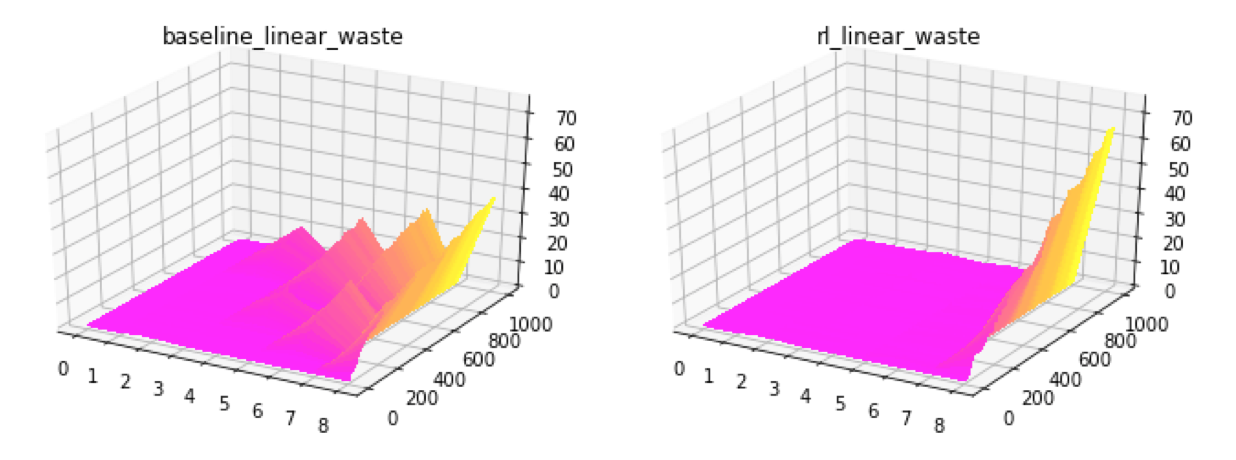
\includegraphics[width=1\linewidth]{images/linear_waste_sol.png}
	\caption{RL vs baseline solution for LW distribution}
	\label{fig:bin_packing_LW_dist}
		\vspace{-1em}
\end{figure}

%\begin{figure}[h!]
%	\centering
%	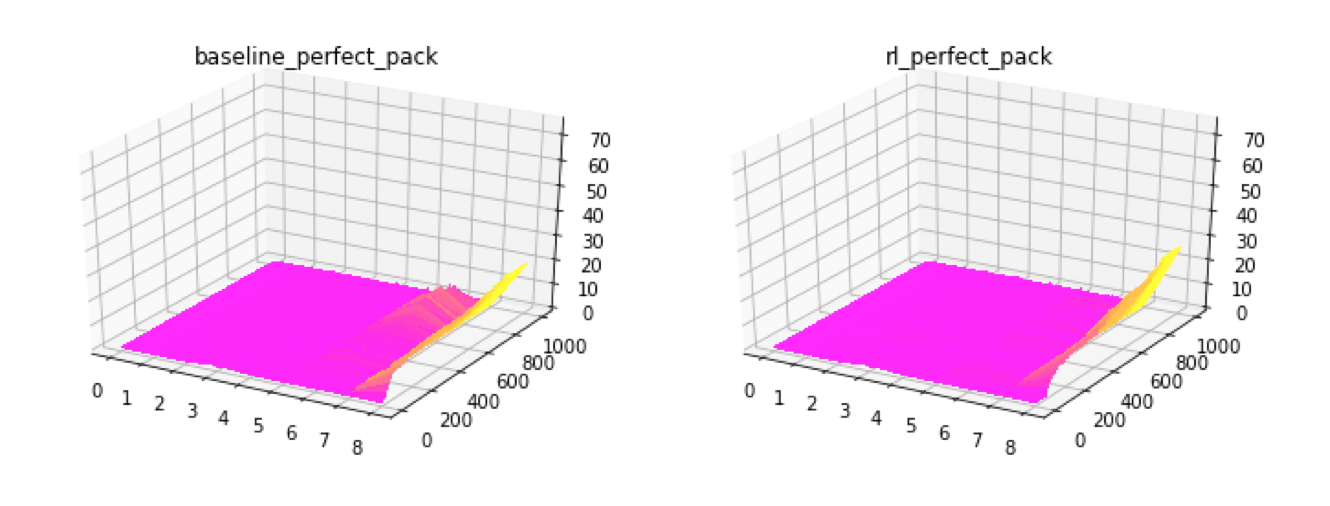
\includegraphics[width=1\linewidth]{images/perfect_packing_sol.png}
%	\caption{RL vs baseline solution for PP distribution}
%	\label{fig:bin_packing_PP_dist}
%\end{figure}
%
%\begin{figure}[h!]
%	\centering
%	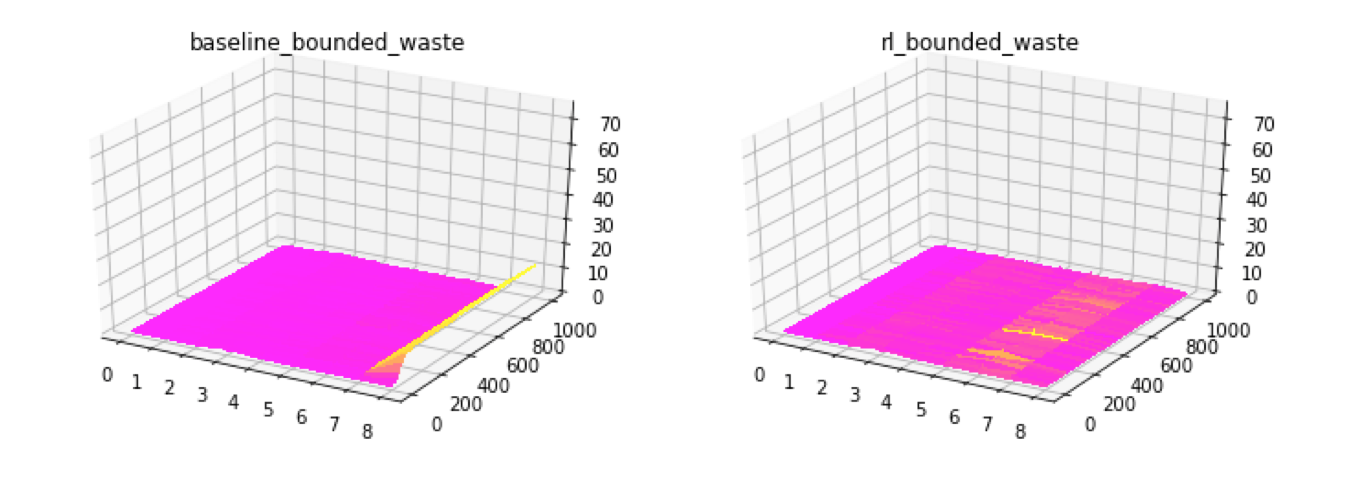
\includegraphics[width=1\linewidth]{images/bounded_waste_sol.png}
%	\caption{RL vs baseline solution for BW distribution}
%	\label{fig:bin_packing_BW_dist}
%\end{figure}

%Note that for all items size distributions, solution returned by RL uses many more bins at fullness level of 8 or 9 (recall that bin size is 9), whereas SS also uses more bins at lower fullness level compared to RL. 
%Below is an example of the frequency of bins of different fullness level for one run of RL vs baseline for each of the three size distributions:
\ifx
\begin{table}[h!]
	\centering
	\begin{tabular}{ |c|cc|cc|cc| } 
			\hline
Fullness Level&LW&&PP&&BW& \\
\hline
& RL&SS&RL&SS&RL&SS \\
\hline

2 & 0 & 1 & 0 & 0 & 0 & 0 \\
\hline
3 & 0 & 0 & 2 & 0 & 0 & 0 \\
\hline
4 & 0 & 9 & 0 & 1 & 0 & 0 \\
\hline
5 & 1 & 0 & 0 & 0 & 0 & 0 \\
\hline
6 & 0 & 16 & 0 & 9 & 0 & 2 \\
\hline
7 & 0 & 0 & 0 & 0 & 1 & 0 \\
\hline
8 & 78 & 27 & 19 & 18 & 0 & 10 \\
\hline
9 & 173 & 208 & 233 & 229 & 278 & 271 \\
\hline
Total Reward & -82 & -127 & -31 & -50 & -2 & -16 \\
		\hline
	\end{tabular}
	\caption{Comparison between RL and baseline solutions.}
	\label{table:bin_packing_RL_baseline_sol_comp}
\end{table}
\fi
\ifx
\begin{table}[h!]
	\centering
	\begin{tabular}{ |c|c|c| } 
		\hline
		Packing Type & RL & SS \\ 
		\hline
		2 & 0 & 1  \\ 
		\hline
		2,2 & 0 & 9 \\
		\hline
		2,3 & 1 & 0 \\
		\hline
		2,2,2 & 0 & 16 \\   
		\hline
		2,2,2,2 & 76 & 26 \\
		\hline
		2,3,3 & 2 & 1 \\
		\hline
		2,2,2,3 & 169 & 206 \\
		\hline
		3,3,3 & 4 & 2 \\
		\hline
		Total Reward & -82 &-127 \\
		\hline
	\end{tabular}
\end{table}

\begin{table}[h!]
	\centering
	\begin{tabular}{ |c|c|c| } 
		\hline
		Packing Type & RL & SS \\ 
		\hline
		3 & 2 & 0 \\
		\hline
		2,2 & 0 & 1 \\
		\hline
		2,2,2 & 0 & 9 \\   
		\hline
		3,3 & 0 & 0 \\
		\hline
		2,3,3 & 3 & 3 \\
		\hline
		2,2,2,2 & 16 & 15 \\
		\hline
		2,2,2,3 & 226  & 215 \\
		\hline
		3,3,3 & 7 & 14 \\
		\hline
		Total Reward & -31 &-50 \\
		\hline
	\end{tabular}
\end{table}

\begin{table}[h!]
	\centering
	\begin{tabular}{ |c|c|c| } 
		\hline
		Packing Type & RL & SS \\ 
		\hline
		2,2,2 & 0 & 1 \\   
		\hline
		3,3 & 0 & 1 \\
		\hline
		2,2,3 & 1 & 0 \\
		\hline
		2,3,3 & 0 & 10 \\
		\hline
		2,2,2,3 & 163 & 152 \\
		\hline
		3,3,3 & 115 & 119 \\
		\hline
		Total Reward & -2 &-16 \\
		\hline
	\end{tabular}
\end{table}
\fi

